\chapter{O SURGIMENTO DO CONCEITO DE LIMITE}
O conceito originário de limite surgiu na Grécia antiga no século V a.C., influenciado pelos paradoxos de Zenão. Os argumentos de Zenão que causaram maior perturbação foram os quatro paradoxos sobre a impossibilidade do movimento, sendo eles: o da Dicotomia, o da Flecha, do Estádio e o de Aquiles.



\medskip
Segundo o paradoxo mais famoso o de Aquiles e a Tartaruga: Aquiles e a tartaruga resolvem apostar uma corrida, como Aquiles é muito mais veloz, decidiu dar uma vantagem a tartaruga que começou num ponto $A$ mais a frente do ponto de largada; o veloz Aquiles corre para alcançar a tartaruga, mas quando chega ao ponto $A$ de onde partiu a tartaruga, esta se encontra mais adiante, numa outra posição $B$. Quando Aquiles chega à posição $B$, a tartaruga também avança para uma nova posição $C$, e assim sucessivamente, de tal forma que Aquiles sempre se aproximará da tartaruga, porém sem nunca alcançá-la.

\medskip

\begin{figure}[H]
\centering % para centralizarmos a figura
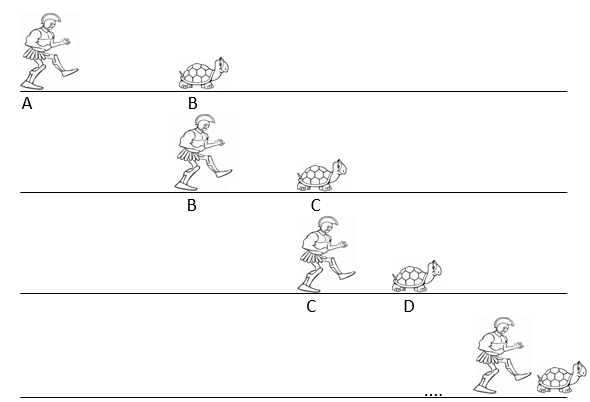
\includegraphics[width=10cm]{img/aquiles.png} % leia abaixo
\caption{Aquiles e a tartaruga.}
\label{fig:aquiles}
\end{figure}


\medskip

As afirmações de Zenão
envolvem conceitos de continuidade do infinito e do infinitesimal, e
são ainda hoje, motivo de debate tanto quanto o foram no tempo de
Aristóteles, que não obteve sucesso ao tentar explicar os paradoxos
de Zenão, onde nenhuma explicação fora satisfatória até a criação do
contínuo e da teoria dos agregados por George Cantor (1845 - 1916
) \cite{cajori}.\\


O trabalho de Eudoxo de Cnido (408 - 355 a. C.), com sua definição
de igualdade de duas razões, constrói uma nova definição de
proporção, de caráter mais geral, utilizando apenas os números
inteiros positivos. Embora tenha sido uma solução genial para a
crise dos incomensuráveis, ele atrasou por mais de mil anos o
desenvolvimento da Aritmética e da Álgebra, pois subordinou essas
disciplinas aos estudos da geometria.\\


\begin{citacao}
Segundo Arquimedes, Eudoxo forneceu o axioma que hoje tem o nome de Arquimedes, às
vezes, chamado axioma de Arquimedes e que serviu de base para o
método de exaustão, o equivalente grego de cálculo integral. O
axioma diz que dadas duas grandezas que têm uma razão (isto é,
nenhuma delas sendo zero), pode-se achar um múltiplo de qualquer
delas que seja maior que a outra. Esse enunciado eliminava um
nebuloso argumento sobre segmentos de reta indivisíveis, ou
infinitésimos fixos, que às vezes aparecia \cite[p.62]{boyer}.
\end{citacao}


\medskip
 Do axioma de Eudoxo (ou Arquimedes) é fácil, por uma redução ao absurdo, provar uma
proposição que formava a base de método de exaustão dos gregos. 
\begin{citacao}
Se de uma grandeza qualquer subtrairmos uma parte não menor que sua
metade e do resto novamente subtrai-se não menor que a metade e se
esse processo de subtração é continuado, finalmente restará uma
grandeza menor que qualquer grandeza de mesma espécie" \cite[p.63]{boyer}. 
\end{citacao}


 De acordo com \citeonline[p.226]{boyer}, Galileu (1564-1642)
tinha tido a intenção de escrever um tratado sobre o infinito em
matemática, mas ele não foi encontrado. Enquanto isso seu discípulo
Cavalieri (1598-1647) fora motivado por Kleper (1571-1630), bem como
por idéias antigas e medievais e pelo encorajamento de Galileu, a
organizar seus pensamentos sobre infinitésimos em formas de livro.
Mas a obra que mais o projetou, é o tratado Geometria
\textit{indivisibilibus}, publicado em sua versão inicial no ano de 1635,
onde apresenta seu método dos indivisíveis.\\


 Merece destaque, a obra de Fermat (1601 - 1665), que de acordo com 
\citeonline[p.239]{boyer} é possível que desde 1629 Fermat já estivesse de posse
da sua Geometria Analítica, pois por essa época ele fez duas
descobertas significativas que se relacionam de perto com seu
trabalho sobre lugares geométricos. A mais importante foi o chamado
"Método para achar máximos e mínimos"   que de acordo com Laplace
(1749 - 1827), lhe rendeu o título de descobridor do Cálculo
Diferencial, bem como co-descobridor da Geometria Analítica.  Afirma 
\citeonline[p.240]{boyer}, que evidentemente Fermat ainda não possuía a definição
formal do conceito de limite, mas por outro lado o seu método para
achar máximos e mínimos se assemelhava muito ao usado hoje no
Cálculo.\\

 No século XVII, surgem
os trabalhos de Isaac Newton (1642 - 1727) e Gottfried Wilhelm
Leibniz (1646 - 1716) que embora tenham tido muitos precursores, a
criação do cálculo, em geral, é atribuídas a eles. No período de
1665-1666,  segundo \citeonline{boyer}, fora o período mais produtivo de
descoberta matemática, pois durante esse período, Newton realizou
quatro de suas principais descobertas: $1.$ O teorema binomial, $2.$ O
cálculo, $3.$ A lei da gravitação e $4.$ A natureza das cores.\\


 Em 1687,
em \textit{Principia Mathematica}, o mais admirado tratado científico de
todos os tempos, Newton tentou dar uma formulação precisa do
conceito de limite: "Quantidades, e as razões de quantidades, que em
qualquer tempo finito convergem continuamente à igualdade, e antes
do fim desse tempo se aproximam mais uma da outra que por qualquer
diferença dada, se tornam finalmente iguais" \cite[p.274]{boyer}. Isto, é claro, é uma
tentativa de definir o limite de uma função.\\


 Segundo \citeonline[p.277]{boyer},
Gottfried Wilhelm Leibniz (1646-1716) inventou seu cálculo entre
1673 e 1676. Usou pela primeira vez o símbolo integral, um S
alongado, derivando da primeira letra da palavra latina \textit{summa} (soma)
em 29 de outubro de 1675. O objetivo era indicar a soma de
indivisíveis. Algumas semanas depois já escrevia diferenciais e
derivadas como o fazemos hoje, assim como escrevia $\displaystyle \int x dy$ e $\displaystyle \int y dx$
para integrais.\\


 Houve uma infeliz polêmica Newton-Leibniz, onde
Leibniz foi acusado de plagiar as descobertas de Newton, mas hoje
não há dúvidas de que ambos criaram o cálculo independentemente.
Embora a descoberta de Newton seja anterior, Leibniz foi o primeiro
a publicar seus resultados.\\


Entretanto, em ambos os cálculos faltavam os fundamentos; tanto
Newton como Leibniz tinham problemas com os infinitesimais, vistos
por ambos de maneira diferentes, mas que operavam de maneiras
parecidas, pois esses infinitesimais às vezes eram cancelados como
fatores diferentes de zero ou desprezados como equivalentes a zero. "Essas operações contraditórias dominaram o cálculo por muito tempo,
até que surgissem trabalhos decisivos para a fundamentação lógica da
disciplina no começo do século XIX" \cite{avila}.\\


 Muito se deve as
contribuições aos membros da família Bernoulli, que no final do
século XVII os irmãos Jacob Bernoulli (1654-1705) e Johann Bernoulli
(1667 - 1748), estavam entre os primeiros matemáticos que perceberam
a potência espantosa do cálculo e aplicaram esse instrumento em uma
gama ampla de problemas.\\


 Johan Bernoulli foi um dos professores mais
inspirado de seu tempo e em troca de um salário regular, forneceu ao
francês de Marquês de l'Hôspital (1661-1704) informações sobre suas
descobertas matemáticas, concedendo a este o direito de usá-las como
lhe conviesse, compondo então seu primeiro texto de cálculo a ser
publicado. Foi assim que o conhecido método de determinação de forma
indeterminada 0/0 tornou-se incorretamente conhecido, em textos
posteriormente de cálculo, como regra de l'Hospital \cite{eves}.\\


D'Alembert (1717-1790), reconheceu explicitamente a importância
central do limite, e em 1754, segundo \citeonline{eves}, fez a mais
importante recomendação de que, para colocar em bases firmes os
fundamentos da análise, era preciso desenvolver uma teoria dos
limites bem estruturada, mas seus contemporâneos quase não lhe deram
ouvidos.\\

Cauchy (1789 - 1875) e Weierstrass (1815 - 1897), dois matemáticos
que merecem destaque, foram fundamentais na busca de uma construção
rigorosa dos fundamentos do Cálculo. Uma das principais
contribuições de Cauchy para o cálculo foi à definição de limite
relativamente clara: "Quando valores sucessivos atribuídos a uma
variável se aproximam indefinidamente de um valor fixo de modo a
acabar diferindo dele tão pouco quanto se queira, este último
chama-se o limite dos outros todos" \cite[p.355]{boyer}.\\

 Enquanto muitos
matemáticos pensavam no infinitésimo como um número fixo muito
pequeno, Cauchy definiu-o claramente como uma variável independente:
"Diz-se que uma quantidade variável se torna infinitamente pequena
quando seu valor numérico diminui indefinidamente de modo a
convergir ao limite zero" \cite[p.355]{boyer}. \\



 No entanto, se buscavam
mais rigor na fundamentação dos números reais, uma vez que a teoria
de limites de Cauchy fora construída sobre uma noção intuitiva
simples do sistema dos números reais. Foi então que, segundo \citeonline{eves}, Weierstrass defendeu um programa no qual o próprio sistema
de números reais fosse tornado mais rigoroso para que assim tudo que
dele decorresse na análise inspirasse segurança, esse notável
programa ficou conhecido como aritmetização da análise, que se
concretizou no final do século XIX com os trabalhos de Richard
Dedeking (1831-1916), George Cantor (1845-1932), os quais permitiram
a demonstração rigorosa dos teoremas fundamentais sobre limites sem
utilizar recursos geométricos, criando dessa forma, uma nova forma
de lógica matemática.\\


Foi assim que, no século XIX, quando segundo \citeonline{avila}, a
definição de limite de Cauchy, correta, porém eivada da noção
espúria de movimento - é agora substituída pela definição puramente
numérica de Weirstrass: \emph{f(x) tem limite L com x tendendo a
$x_{0}$ significa que dado qualquer $\varepsilon>0$, existe
$\delta>0$ tal que se
$0<|x-x_0|<\delta\Rightarrow|f(x)-L|<\varepsilon$.}
